\documentclass[conference]{IEEEtran}
\usepackage{amsmath,amssymb,graphicx,booktabs,url,cite}
\graphicspath{{results/figures/}}
\title{Reproducing and Critiquing Secure Beamforming for MISO Visible Light Communications With Multipath}
\author{\IEEEauthorblockN{Wei Shuwen, Li Su, and Lu Zipeng}
\IEEEauthorblockA{School of Computer Science\\Nanjing University of Information Science and Technology\\Nanjing, China}}
\begin{document}
\maketitle
\begin{abstract}
Wang et al. investigate optical beamforming with reflected paths, inter-symbol interference and uncertain channel information. This report independently implements their secrecy-rate objective and examines its physical interpretation, optimization argument and numerical reproducibility. Five experiment families are regenerated using explicitly specified optical assumptions. The perfect-channel result at a normalized 20 dB is 2.579 bit/s/Hz, close to an approximate published value of 2.58, while other curves differ. A constructive counterexample challenges the claimed independent decomposition. These results support the usefulness of multipath-aware design but qualify claims of global optimality and general interference removal. Missing parameters prevent an exact replay of the published simulations.
\end{abstract}
\begin{IEEEkeywords}
Visible light communication, physical-layer security, beamforming, reproducibility, robust optimization.
\end{IEEEkeywords}

\section{Introduction}
This critique follows the official IEEE conference template~\cite{template}. The reviewed letter~\cite{wang} considers a ceiling transmitter with multiple LED fixtures, a legitimate receiver Bob and an eavesdropper Eve. Its contribution is to incorporate non-line-of-sight (NLoS) reflections and inter-symbol interference (ISI) into perfect-CSI and robust beamforming designs. This is relevant because optimizing a direct-path model can miss security consequences of weaker reflected components.

A useful critique should distinguish the research question, modeling assumptions, mathematical justification and evidence. We therefore inspect the equations, reconstruct the channel under declared assumptions, compare numerical trends and test a specific optimality claim. The accompanying Python package contains executable simulations, parameter records, solver diagnostics and generated data. Its output is an assumption-conditioned reproduction, not the authors' original implementation or experimental dataset.

\section{Related Work}
The letter adopts a Barry-style diffuse-reflection channel associated with indoor VLC modeling~\cite{lee}. Its literature review positions the contribution relative to direct-path secure beamforming and earlier multipath-security studies. Combining channel memory, spatial weights and uncertainty is a useful extension, although each component requires an explicit operational interpretation. Our independent optimization uses fractional programming~\cite{dinkelbach} and convex subproblems implemented with CVXPY~\cite{cvxpy}. These tools evaluate the stated objective without relying on the disputed independent decomposition.

\section{Methodology}
\subsection{Objective and independent solution}
For tap $s$, let $\mathbf b_s,\mathbf e_s$ denote Bob's and Eve's channel rows and $\mathbf w_s$ the beamforming column. Equations (8)--(10) consistently use sums of squared responses. With normalized noise constant $c=3\pi e\,10^{-\gamma/10}$, we optimize
\begin{equation}
 F(W)=\frac{6\sum_s(\mathbf b_s\mathbf w_s)^2+c}
 {\pi e\sum_s(\mathbf e_s\mathbf w_s)^2+c},\quad
 R=\left[\tfrac12\log_2 F(W)\right]^+,
\end{equation}
subject to $\|\mathbf w_s\|_p\leq1$, $p\in\{1,2,\infty\}$. Here $\gamma$ is the normalized SNR parameter, not a separately calibrated physical receiver SNR.

Dinkelbach iterations maximize the numerator minus a trial ratio times the denominator. The resulting tap subproblems are separable. For $p=2$, their solution follows the largest eigenvalue; for $p=1,\infty$, enumeration of projected polytope edges solves the rank-two quadratic. This separability applies to each fractional-programming iteration, rather than to independently optimized rate ratios.

For independent Euclidean uncertainty balls, the exact worst-case response magnitudes are
\begin{align}
 B_s&=\max\{|\mathbf b_s\mathbf w_s|-\epsilon_B\|\mathbf w_s\|_2,0\},\\
 E_s&=|\mathbf e_s\mathbf w_s|+\epsilon_E\|\mathbf w_s\|_2.
\end{align}
The robust solver uses second-order cone subproblems after fixing Bob's response sign. Zero is feasible, and maximizing a nonnegative square-root surrogate gives the maximal tap quadratic. Numerical residuals and solver status are retained; an inaccurate status is not treated as a strict certificate.

\subsection{Parameters and reproducibility boundaries}
We retain the reported $10\times10\times5$ m room, four fixtures, 25 LEDs per fixture, 2.6 W per LED, detector area $1$ cm$^2$, and Bob/Eve positions $(2,0,0)$ and $(-2,0,0)$ m. Table~\ref{tab:params} lists additional assumptions. They are choices needed to run the model, not values supplied by the authors.
\begin{table}[t]
\caption{Additional implementation assumptions}\label{tab:params}
\centering\begin{tabular}{ll}\toprule
Parameter & Adopted value\\\midrule
Fixture centres & $(\pm2.5,\pm2.5,5)$ m\\
LED arrangement & $5\times5$, pitch 0.1 m\\
Half-power angle / receiver FoV & $60^\circ /85^\circ$\\
Responsivity / refractive index & 0.53 A/W / 1.5\\
Wall reflectivity & 0.6, wavelength independent\\
Wall element / time resolution & 1 m / 0.5 ns\\
Symbol period / available taps & 10 ns / 50\\
Reflecting surfaces & Four vertical walls\\\bottomrule
\end{tabular}
\end{table}

Diffuse energy is propagated deterministically between wall-element centres, including flight delays and up to six reflections. Floor and ceiling reflections are omitted. All channels share one normalization factor: the Euclidean norm of nominal Bob's direct-path first tap. Thus the horizontal axis represents $20\log_{10}(\alpha g_{\rm ref}/\sigma_{\rm physical})$. This normalization is disclosed because the published numerical paragraph does not explain how optical gains and its 0--20 dB axis are reconciled.

The source also omits fixture coordinates, symbol timing, additional-user locations and the mapping from positional uncertainty to channel-radius bounds. We use fixed-seed nested user sets in opposite room halves. Our multiuser experiment implements the published per-tap extrema literally. Robust curves show independent-ball worst-case rates; a separate position experiment uses 1000 uniformly sampled Eve locations inside an assumed 0.25 m disk. These are distinct uncertainty experiments.

\section{Results and Discussion}
\subsection{Reproduced mechanisms and quantitative comparison}
Fig.~\ref{fig:map} regenerates the spatial SNR experiment, while Fig.~\ref{fig:results} covers the other four plot families. Optimized weights suppress reception near Eve. Increasing the normalized SNR generally raises secrecy rate, and zero forcing approaches the perfect-CSI optimum at high SNR. Additional Bob candidates improve the published selection objective, while additional Eve candidates reduce it. Larger uncertainty balls reduce the robust optimum. These mechanisms agree with the main reported trends.
\begin{figure}[t]\centering
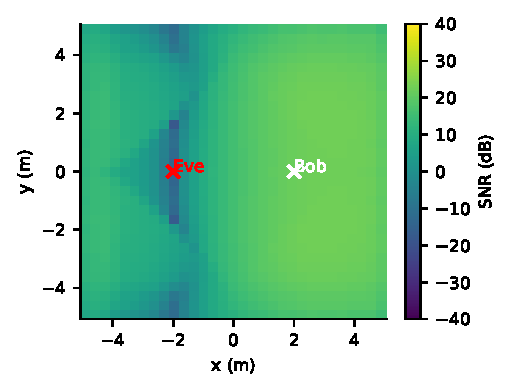
\includegraphics[width=\columnwidth]{report_map.pdf}
\caption{Independent analogue of the paper's Fig. 2, using the declared channel and a fixed optimized beamformer.}\label{fig:map}
\end{figure}
\begin{figure*}[t]\centering
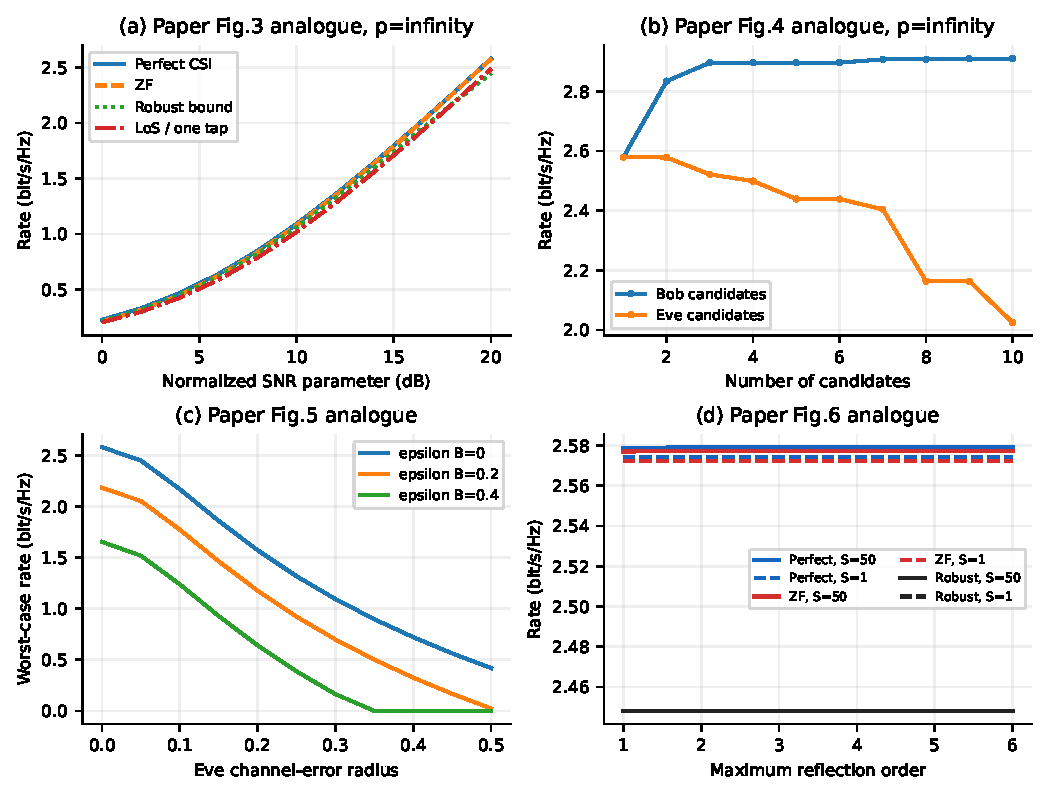
\includegraphics[width=\textwidth]{report_results.pdf}
\caption{Independent analogues of the paper's Figs. 3--6. Shown results use $p=\infty$; the executable package also evaluates $p=1,2$. Curves are computed outputs under declared assumptions, not digitized publication curves.}\label{fig:results}
\end{figure*}

Table~\ref{tab:compare} compares representative 20 dB results with approximate readings of the paper's Fig. 3. The close perfect-CSI endpoint alone does not validate the entire reconstruction: the direct-path baseline differs substantially, and robust quantities use different evaluation procedures. Source readings have approximately $\pm0.03$ bit/s/Hz graphical uncertainty; they are not author-supplied raw data. No optical parameter was fitted to these points.
\begin{table}[t]\caption{Representative comparison, $p=\infty$, 20 dB}\label{tab:compare}\centering
\begin{tabular}{lrr}\toprule
Scheme & Paper reading & Computed\\\midrule
Perfect CSI, multipath & 2.58 & 2.579\\
Zero forcing, multipath & 2.54 & 2.577\\
Robust, $\epsilon_E=0.05$ & 2.37 & 2.448\\
Direct path, one tap & 2.25 & 2.487\\\bottomrule
\end{tabular}
\end{table}

Reflections improve some rates, but the improvement and saturation depend on the channel assumptions. We separately retain a DC baseline that integrates all reflected energy: truncating to one tap is not equivalent to removing ISI while preserving received energy. Consequently, the paper's observation about larger $S$ cannot establish that arbitrary physical ISI is harmless. Equation (8) assumes separate parallel components and combining; implementability and overhead deserve additional analysis.

The 1000-position stress test gives mean rate 2.5549 and minimum 2.4937 bit/s/Hz, compared with the designed bound 2.4481. Only 65.9\% of sampled channels satisfy the chosen per-tap radius 0.05. The observed minimum exceeds the bound, but the guarantee applies only to channels within the uncertainty set. A radius must therefore be calibrated to location errors before making deployment claims.

\subsection{Verification and numerical limitations}
Tests cover an analytic Eve-free solution, identical-channel zero secrecy, zero-forcing nulls, norm feasibility, norm-ball nesting, a dense-grid quadratic comparison, uncertainty monotonicity and sampled worst-case inequalities. The nominal Bob DC-gain vector differs by 0.472\% between 1 m and 0.5 m wall meshes. This checks one spatially integrated quantity; it does not establish universal temporal or spatial convergence.

The run generated 303 solver records. Seven robust records included an \texttt{optimal\_inaccurate} subproblem status, with maximum recorded cone violation below $2.9\times10^{-9}$ and fractional relative residual below $8.2\times10^{-9}$. These diagnostics support numerical consistency while preserving the status qualification. Fixed seeds, raw arrays and CSV outputs permit independent reruns.

\subsection{A constructive optimality counterexample}
Proposition 1 argues that independent beamforming columns permit independent subproblems. Independent feasible sets alone do not establish this for a ratio of sums. Let $N_F=4$, $S=2$, $p=\infty$, $\alpha=\sigma=1$, and $\mathbf a=(1,1,1,1)/4$. Choose
\begin{equation}
\mathbf b_1=3\mathbf a,\quad\mathbf b_2=\mathbf a,\quad
\mathbf e_1=0.1\mathbf a,\quad\mathbf e_2=0.7\mathbf a.
\end{equation}
All channel coefficients are positive. The minimum leakage ratios are $1/30$ and $0.7$, both below $\sqrt{6/(\pi e)}$. For every permitted ratio, equation (13) maximizes each Bob amplitude by setting both columns to the all-ones vector. This yields 0.759158 bit/s/Hz. Setting the second column to zero is feasible and yields 0.815545. Because the objective is linear-fractional in the two squared effective amplitudes, checking their four boundary corners verifies the improved global value. The example invalidates a general optimality justification; it does not establish that every plotted solution is suboptimal.

\subsection{Further interpretive qualifications}
Algorithm 1 specifies a dB condition on $\Delta\beta_s$ but subsequently adds it in linear units. With the stated 0.2 dB tolerance, that condition implies a linear increment above one, despite the search upper bound being approximately 0.838. A reproducible implementation needs the intended units clarified.

Equations (14)--(15) also place receiver extrema inside the tap sum. Generally, $\sum_s\max_j P_{js}\neq\max_j\sum_sP_{js}$. For two receivers with tap powers $(4,1)$ and $(1,4)$, these give eight and five. Per-tap receiver selection needs explicit justification when describing one selected receiver or one worst non-colluding eavesdropper. Finally, the unit-radius norm balls are nested, so superior $p=\infty$ performance does not demonstrate superiority under equal optical budgets.

\section{Conclusion}
The paper makes a useful case for considering reflections, temporal components and uncertainty together. Our executable reconstruction supports several qualitative trends and exposes the limits of exact numerical reproducibility. Its strongest qualifications concern the independent-decomposition argument, uncertainty calibration and multiuser selection semantics. Publishing complete channel parameters, author code and raw results would make the conclusions more testable. The delivered reproduction should be interpreted as an independent, assumption-conditioned evaluation of the stated model, with explicit differences from the published simulations.

\begin{thebibliography}{5}
\bibitem{template} IEEE, ``Conference templates.'' [Online]. Available: \url{https://www.ieee.org/conferences/publishing/templates.html}
\bibitem{wang} J.-Y. Wang, Y.-C. Yu, D.-S. Lu, and D.-P. Su, ``Secure beamforming for MISO visible light communications with ISI and NLoS components,'' \emph{IEEE Wireless Commun. Lett.}, vol. 13, no. 3, pp. 908--912, 2024, doi: 10.1109/LWC.2024.3350544.
\bibitem{lee} K. Lee, H. Park, and J. R. Barry, ``Indoor channel characteristics for visible light communications,'' \emph{IEEE Commun. Lett.}, vol. 15, no. 2, pp. 217--219, 2011.
\bibitem{dinkelbach} W. Dinkelbach, ``On nonlinear fractional programming,'' \emph{Management Science}, vol. 13, no. 7, pp. 492--498, 1967.
\bibitem{cvxpy} S. Diamond and S. Boyd, ``CVXPY: A Python-embedded modeling language for convex optimization,'' \emph{J. Mach. Learn. Res.}, vol. 17, no. 83, pp. 1--5, 2016.
\end{thebibliography}
\end{document}
